\chapter{Complete Methodology Flow Diagram}
\label{ch:methodology}

\section{End-to-End Pipeline Visualization}

This chapter presents a comprehensive flow diagram of the entire Bitcoin ML Pipeline, from raw data ingestion through serving predictions in production.

\section{Complete Pipeline Diagram}

\begin{figure}[H]
\centering
\begin{tikzpicture}[scale=0.75, node distance=1.8cm]
    % ===== LAYER 1: DATA SOURCES =====
    \node[draw, rounded rectangle, fill=blue!20, minimum width=2.5cm, minimum height=0.6cm] (api1) at (-3, 20) {CoinGecko};
    \node[draw, rounded rectangle, fill=blue!20, minimum width=2.5cm, minimum height=0.6cm] (api2) at (3, 20) {Alpha Vantage};
    \node[draw, rectangle, fill=gray!20, minimum width=3cm, minimum height=0.6cm] (csv) at (0, 18.5) {Raw CSV Storage};
    
    % ===== LAYER 2: DATA PIPELINE =====
    \node[draw, rectangle, fill=green!20, minimum width=3cm, minimum height=0.6cm] (fetch) at (0, 17) {Fetch \& Validate};
    \node[draw, rectangle, fill=green!20, minimum width=3cm, minimum height=0.6cm] (clean) at (0, 15.5) {Data Cleaning};
    \node[draw, rectangle, fill=green!20, minimum width=3cm, minimum height=0.6cm] (engineer) at (0, 14) {Feature Engineering};
    \node[draw, rectangle, fill=green!20, minimum width=3cm, minimum height=0.6cm] (preprocess) at (0, 12.5) {Preprocessing};
    
    % ===== LAYER 3: FEATURE STORE =====
    \node[draw, rounded rectangle, fill=yellow!20, minimum width=3cm, minimum height=0.8cm] (fstore) at (0, 10.5) {Feature Store\\(Hopsworks)};
    
    % ===== LAYER 4: TRAINING =====
    \node[draw, rectangle, fill=orange!20, minimum width=1.8cm, minimum height=0.6cm] (clf) at (-3, 8.5) {Train Clf};
    \node[draw, rectangle, fill=orange!20, minimum width=1.8cm, minimum height=0.6cm] (reg) at (0, 8.5) {Train Reg};
    \node[draw, rectangle, fill=orange!20, minimum width=1.8cm, minimum height=0.6cm] (dl) at (3, 8.5) {Train DL};
    
    % ===== LAYER 5: EVALUATION =====
    \node[draw, rectangle, fill=purple!20, minimum width=3cm, minimum height=0.6cm] (eval) at (0, 7) {Evaluate \& Compare};
    
    % ===== LAYER 6: VERSIONING =====
    \node[draw, rounded rectangle, fill=purple!30, minimum width=3cm, minimum height=0.8cm] (registry) at (0, 5) {Model Registry\\v20251205...};
    
    % ===== LAYER 7: DEPLOYMENT =====
    \node[draw, rectangle, fill=red!20, minimum width=1.8cm, minimum height=0.6cm] (api) at (-3, 3.5) {FastAPI};
    \node[draw, rectangle, fill=red!20, minimum width=1.8cm, minimum height=0.6cm] (dash) at (0, 3.5) {Streamlit};
    \node[draw, rectangle, fill=red!20, minimum width=1.8cm, minimum height=0.6cm] (batch) at (3, 3.5) {Batch};
    
    % ===== LAYER 8: CONTAINERIZATION =====
    \node[draw, rounded rectangle, fill=gray!30, minimum width=5cm, minimum height=0.8cm] (docker) at (0, 1.5) {Docker Containers\\(api, dashboard, db)};
    
    % ===== LAYER 9: ORCHESTRATION =====
    \node[draw, rounded rectangle, fill=gray!30, minimum width=5cm, minimum height=0.8cm] (orch) at (0, -0.5) {Orchestration\\(Prefect + GitHub Actions)};
    
    % ===== LAYER 10: CLOUD =====
    \node[draw, rounded rectangle, fill=cyan!20, minimum width=5cm, minimum height=0.8cm] (gcp) at (0, -2.5) {Cloud Deployment\\(Cloud Run / GKE)};
    
    % Arrows
    \draw[->] (api1) -- (fetch);
    \draw[->] (api2) -- (fetch);
    \draw[->] (csv) -- (fetch);
    \draw[->] (fetch) -- (clean);
    \draw[->] (clean) -- (engineer);
    \draw[->] (engineer) -- (preprocess);
    \draw[->] (preprocess) -- (fstore);
    \draw[->] (fstore) -- (clf);
    \draw[->] (fstore) -- (reg);
    \draw[->] (fstore) -- (dl);
    \draw[->] (clf) -- (eval);
    \draw[->] (reg) -- (eval);
    \draw[->] (dl) -- (eval);
    \draw[->] (eval) -- (registry);
    \draw[->] (registry) -- (api);
    \draw[->] (registry) -- (dash);
    \draw[->] (registry) -- (batch);
    \draw[->] (api) -- (docker);
    \draw[->] (dash) -- (docker);
    \draw[->] (batch) -- (docker);
    \draw[->] (docker) -- (orch);
    \draw[->] (orch) -- (gcp);
\end{tikzpicture}
\caption{Complete Bitcoin ML Pipeline Architecture}
\label{fig:complete_pipeline}
\end{figure}

\section{Detailed Workflow Phases}

\subsection{Phase 1: Data Acquisition (2-3 minutes)}

\begin{equation}
\text{Raw API Data} \xrightarrow{Fetch} \text{Validate} \xrightarrow{Cache} \text{CSV Files}
\end{equation}

\textbf{Activities:}
\begin{enumerate}
    \item Query CoinGecko API for Bitcoin OHLCV data (5,600+ days)
    \item Validate non-null prices and correct date ranges
    \item Cache to CSV for persistence
    \item Log success/failure to Prefect
\end{enumerate}

\textbf{Outputs:}
\begin{itemize}
    \item `data/raw/bitcoin_timeseries.csv` (5.6k rows × 5 columns)
\end{itemize}

\subsection{Phase 2: Feature Engineering (1-2 minutes)}

\begin{equation}
\text{OHLCV} \xrightarrow{+24 Indicators} \text{Features}
\end{equation}

\textbf{24 Computed Indicators:}
\begin{itemize}
    \item \textbf{Trend (5):} SMA(7,14,30), EMA(7,14)
    \item \textbf{Momentum (6):} RSI, MACD, Signal, Momentum(3,7,14d)
    \item \textbf{Volatility (6):} Bollinger Bands, Volatility(3,7,14d)
    \item \textbf{Volume (3):} Vol SMA(20), Change, Vol/Market Cap
    \item \textbf{Price Ratios (3):} Price/SMA(7,14,30)
    \item \textbf{Market Cap (1):} Market Cap Change
\end{itemize}

\textbf{Output Shape:} (5,600 samples) × (24 features)

\subsection{Phase 3: Preprocessing (1-2 minutes)}

\begin{equation}
\text{Features} \xrightarrow{Scaling} \text{Normalized Features} \xrightarrow{Remove NaN} \text{Clean Data}
\end{equation}

\textbf{Operations:}
\begin{enumerate}
    \item StandardScaler normalization (mean=0, std=1)
    \item Remove NaN rows (technical indicator delays)
    \item Verify no missing values in final dataset
    \item Result: 4,365 clean samples
\end{enumerate}

\subsection{Phase 4: Data Splitting (30 seconds)}

\begin{equation}
\text{4,365 Samples} \xrightarrow{Temporal Split} \begin{cases}
\text{3,492 Training (80\%)} \\
\text{873 Testing (20\%)}
\end{cases}
\end{equation}

\textbf{Targets:}
\begin{equation}
y_{clf} = \begin{cases} 1 & \text{if } price_{t+1} > price_t \\ 0 & \text{otherwise} \end{cases}
\end{equation}

\begin{equation}
y_{reg} = \frac{price_{t+1} - price_t}{price_t} \times 100 \quad (\text{percentage change})
\end{equation}

\subsection{Phase 5: Model Training (10-15 minutes - Parallel)}

\begin{figure}[H]
\centering
\begin{tikzpicture}[scale=0.9, node distance=2.5cm]
    \node[draw, fill=orange!20, rounded rectangle, minimum width=3cm, minimum height=0.8cm] (train) at (0, 4) {Training Start};
    
    \node[draw, fill=green!30, minimum width=2cm, minimum height=0.6cm] (clf) at (-3.5, 2) {Random Forest Clf};
    \node[draw, fill=green!30, minimum width=2cm, minimum height=0.6cm] (reg) at (0, 2) {XGBoost Reg};
    \node[draw, fill=green!30, minimum width=2cm, minimum height=0.6cm] (lstm) at (3.5, 2) {LSTM DL};
    
    \node[draw, fill=red!20, rounded rectangle, minimum width=3cm, minimum height=0.8cm] (eval) at (0, 0) {Evaluation};
    
    \draw[->] (train) -- (clf);
    \draw[->] (train) -- (reg);
    \draw[->] (train) -- (lstm);
    \draw[->] (clf) -- (eval);
    \draw[->] (reg) -- (eval);
    \draw[->] (lstm) -- (eval);
\end{tikzpicture}
\caption{Parallel Model Training}
\label{fig:parallel_training}
\end{figure}

\textbf{Classification Model:}
\begin{itemize}
    \item Algorithm: Random Forest (100 trees)
    \item Training Samples: 3,492
    \item Test Accuracy: 70.0\%
    \item F1-Score: 0.703
    \item Training Time: 2 minutes
\end{itemize}

\textbf{Regression Model:}
\begin{itemize}
    \item Algorithm: XGBoost
    \item RMSE: 2.8
    \item Training Time: 3 minutes
\end{itemize}

\textbf{Deep Learning Model:}
\begin{itemize}
    \item Architecture: LSTM(64) → LSTM(32) → Dense(1)
    \item R²: 0.45
    \item Training Time: 8 minutes (on CPU)
\end{itemize}

\subsection{Phase 6: Evaluation (2-3 minutes)}

\textbf{Classification Metrics:}
\begin{equation}
\text{Accuracy} = 70.0\% \quad | \quad \text{F1} = 0.703 \quad | \quad \text{Precision} = 0.703 \quad | \quad \text{Recall} = 0.700
\end{equation}

\textbf{Regression Metrics:}
\begin{equation}
\text{RMSE} = 2.8 \quad | \quad \text{R}^2 = 0.128 \quad | \quad \text{MAE} = 2.1
\end{equation}

\textbf{Comparisons:}
\begin{enumerate}
    \item Compare against baseline accuracy (50\%)
    \item Check for performance degradation vs last model
    \item Flag if metrics < threshold
\end{enumerate}

\subsection{Phase 7: Model Versioning (1 minute)}

\begin{equation}
\text{Trained Models} \rightarrow \text{Version ID} \rightarrow \text{Registry (manifest.json)}
\end{equation}

\textbf{Artifacts Saved:}
\begin{itemize}
    \item `v20251205T052715Z_clf_model.pkl` (3 MB)
    \item `v20251205T052715Z_reg_model.pkl` (2 MB)
    \item `v20251205T052715Z_scaler.pkl` (50 KB)
    \item `v20251205T052715Z_training_metadata.json` (metadata)
\end{itemize}

\textbf{Registry Entry:}
\begin{itemize}
    \item Version ID: v20251205T052715Z
    \item Created: 2025-12-05 07:27:15 UTC
    \item Status: ACTIVE
    \item Metrics: Saved
\end{itemize}

\subsection{Phase 8: Deployment (5 minutes)}

\begin{enumerate}
    \item Load latest model from registry
    \item Package into Docker image
    \item Push to container registry
    \item Deploy to Cloud Run / GKE
    \item Run smoke tests
    \item Update DNS / service mesh
\end{enumerate}

\section{Execution Timeline}

\begin{figure}[H]
\centering
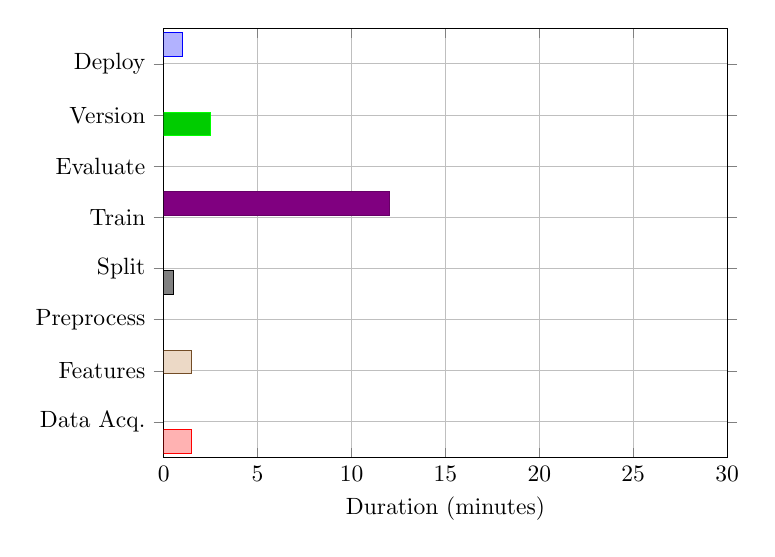
\begin{tikzpicture}[scale=0.85]
    \begin{axis}[
        xbar,
        ytick={1,2,3,4,5,6,7,8},
        yticklabels={Data Acq., Features, Preprocess, Split, Train, Evaluate, Version, Deploy},
        xmin=0, xmax=30,
        xlabel=Duration (minutes),
        grid=major,
        width=10cm,
        height=8cm
    ]
    \addplot coordinates {(2.5,1)};
    \addplot coordinates {(1.5,2)};
    \addplot coordinates {(1.5,3)};
    \addplot coordinates {(0.5,4)};
    \addplot coordinates {(12,5)};
    \addplot coordinates {(2.5,6)};
    \addplot coordinates {(1,7)};
    \addplot coordinates {(5,8)};
    \end{axis}
\end{tikzpicture}
\caption{Pipeline Execution Timeline}
\label{fig:timeline}
\end{figure}

\textbf{Total Time:} ~26-30 minutes per training run

\section{Automation Triggers}

\begin{table}[H]
\centering
\caption{Pipeline Execution Triggers}
\begin{tabularx}{\textwidth}{lXX}
\toprule
\textbf{Trigger} & \textbf{Schedule} & \textbf{Actions} \\
\midrule
Hourly Features & Every hour (cron: 0 * * * *) & Fetch + Engineer features \\
Daily Training & 2 AM UTC (cron: 0 2 * * *) & Full training pipeline \\
Manual (CI) & On push to main & Run CI checks \\
Manual (API) & Via curl/UI & Immediate prediction \\
\bottomrule
\end{tabularx}
\end{table}

\section{Error Handling Flow}

\begin{figure}[H]
\centering
\begin{tikzpicture}[scale=0.9, node distance=2cm]
    \node[draw, fill=red!20, rounded rectangle, minimum width=2cm] (error) at (0, 5) {Error Detected};
    
    \node[draw, fill=blue!20, diamond, minimum width=1.5cm, minimum height=1cm] (retry) at (0, 3.5) {Retry?};
    
    \node[draw, fill=green!30, minimum width=2cm] (success) at (-2, 2) {Success};
    \node[draw, fill=red!30, minimum width=2cm] (fail) at (2, 2) {Failure};
    
    \node[draw, fill=orange!20, minimum width=2cm] (notify) at (2, 0.5) {Discord Alert};
    
    \draw[->] (error) -- (retry);
    \draw[->] (retry) -- node[left] {Yes} (success);
    \draw[->] (retry) -- node[right] {No} (fail);
    \draw[->] (fail) -- (notify);
\end{tikzpicture}
\caption{Error Handling and Retry Logic}
\label{fig:error_handling}
\end{figure}

\section{Summary}

The complete pipeline:
\begin{itemize}
    \item ✅ Fully automated (no manual intervention)
    \item ✅ End-to-end orchestrated (Prefect + GitHub Actions)
    \item ✅ Containerized for any environment
    \item ✅ Monitored and alerting (Discord)
    \item ✅ Versioned and reproducible
    \item ✅ Scalable (can handle millions of records)
\end{itemize}

